%!TEX program=xelatex
% 注意事项:编译两次,以确保目录、页码完整显示
% 华东师范大学软件工程学院课程报告
% https://github.com/Shichien/ECNU-LateX-Template
% Author - 10235101526

\def\allfiles{}

\documentclass[14pt,a4paper,UTF8,twoside]{article}

% Title Page ————————————————————————————————————————
\usepackage{setspace}

% Formatting Packages ——————————————————————————————————————
\usepackage{multicol}
\usepackage{multirow}
\usepackage{enumitem}
\usepackage{indentfirst}

% Math & Physics Packages ————————————————————————————
\usepackage{amsmath, amsthm, amsfonts, amssymb}
\usepackage{physics}
\usepackage{cancel}
\usepackage{nicefrac}
\usepackage{unicode-math} % 允许数学公式使用特定字体
\usepackage{mdframed}
\usepackage{forest}

% Image-related Packages —————————————————————————————
\usepackage{float} % 浮动体环境
\usepackage{subcaption} % 子图包
\usepackage{pgfgantt}
\usepackage{graphics, graphicx}
\usepackage{tikz, tikz-qtree}
\usetikzlibrary{arrows.meta, positioning, fit, shapes}
\usetikzlibrary{shapes.geometric}
\tikzstyle{node_style} = [rectangle, rounded corners, draw, align=center, text width=3cm, minimum height=0.65cm]
\tikzstyle{arrow_style} = [thick, ->, >=stealth]

\usepackage{pgfplots}
\pgfplotsset{compat=1.18}
\usepackage{xcolor}
\usepackage{fourier-orns}
\usepackage{lipsum}

% Colour Palette ——————————————————————————————————————
\definecolor{merah}{HTML}{F4564E}
\definecolor{merahtua}{HTML}{89313E}
\definecolor{biru}{HTML}{60BBE5}
\definecolor{birutua}{HTML}{412F66}
\definecolor{hijau}{HTML}{59CC78}
\definecolor{hijautua}{HTML}{366D5B}
\definecolor{kuning}{HTML}{FFD56B}
\definecolor{jingga}{HTML}{FBA15F}
\definecolor{ungu}{HTML}{8C5FBF}
\definecolor{lavender}{HTML}{CBA5E8}
\definecolor{merjamb}{HTML}{FFB6E0}
\definecolor{mygray}{HTML}{E6E6E6}
\definecolor{mygreen}{rgb}{0,0.6,0}
\definecolor{mymauve}{rgb}{0.58,0,0.82}

% Theorems ————————————————————————————————————————————
\usepackage{tcolorbox}
\usepackage{changepage}
\tcbuselibrary{skins,breakable,theorems}

\newcounter{hitung}
\setcounter{hitung}{\thesection}

\makeatletter
% Proof 证明如下
\def\tcb@theo@widetitle#1#2#3{\hbox to \textwidth{\textsc{\large#1}\normalsize\space#3\hfil(#2)}}
\tcbset{
    theorem style/theorem wide name and number/.code={ \let\tcb@theo@title=\tcb@theo@widetitle},
    proofbox/.style={skin=enhancedmiddle,breakable,parbox=false,boxrule=0mm,
    check odd page, toggle left and right, colframe=black!20!white!92!hijau,
    leftrule=8pt, rightrule=0mm, boxsep=0mm,arc=0mm, outer arc=0mm,
    left=3mm,right=3mm,top=0mm,bottom=0mm, toptitle=0mm,
    bottomtitle=0mm,colback=gray!3!white!98!biru, before skip=8pt, after skip=8pt,
    before={\par\vskip-2pt},after={\par\smallbreak},
    },
}
\newtcolorbox{ProofBox}{proofbox}
\makeatother

\let\realproof\proof
\let\realendproof\endproof
\renewenvironment{proof}[1][Prove:]{\ProofBox\strut\textsc{#1}\space}{\endProofBox}
\AtEndEnvironment{proof}{\null\hfill$\blacksquare$}
% Definition 定义环境
\newtcbtheorem[use counter=hitung, number within=section]{dfn}{定义}
{theorem style=theorem wide name and number,breakable,enhanced,arc=3.5mm,outer arc=3.5mm,
    boxrule=0pt,toprule=1pt,leftrule=0pt,bottomrule=1pt, rightrule=0pt,left=0.2cm,right=0.2cm,
    titlerule=0.5em,toptitle=0.1cm,bottomtitle=-0.1cm,top=0.2cm,
    colframe=white!10!biru,
    colback=white!90!biru,
    coltitle=white,
    shadow={1.3mm}{-1.3mm}{0mm}{gray!50!white}, % 添加阴影
    coltext=birutua!60!gray, title style={white!10!biru}, before skip=8pt, after skip=8pt,
    fonttitle=\bfseries,fontupper=\normalsize}{dfn}

% 答题卡
\newtcbtheorem[use counter=hitung, number within=section]{ans}{解答}
{theorem style=theorem wide name and number,breakable,enhanced,arc=3.5mm,outer arc=3.5mm,
    boxrule=0pt,toprule=1pt,leftrule=0pt,bottomrule=1pt, rightrule=0pt,left=0.2cm,right=0.2cm,
    titlerule=0.5em,toptitle=0.1cm,bottomtitle=-0.1cm,top=0.2cm,
    colframe=white!10!biru,
    colback=white!90!biru,
    coltitle=white,
    shadow={1.3mm}{-1.3mm}{0mm}{gray!50!white}, % 添加阴影
    coltext=birutua!60!gray, title style={white!10!biru}, before skip=8pt, after skip=8pt,
    fonttitle=\bfseries,fontupper=\normalsize}{ans}

% Axiom
\newtcbtheorem[use counter=hitung, number within=section]{axm}{公理}
{theorem style=theorem wide name and number,breakable,enhanced,arc=3.5mm,outer arc=3.5mm,
    boxrule=0pt,toprule=1pt,leftrule=0pt,bottomrule=1pt, rightrule=0pt,left=0.2cm,right=0.2cm,
    titlerule=0.5em,toptitle=0.1cm,bottomtitle=-0.1cm,top=0.2cm,
    colframe=white!10!biru,colback=white!90!biru,coltitle=white,
    shadow={1.3mm}{-1.3mm}{0mm}{gray!50!white!90}, % 添加阴影
    coltext=birutua!60!gray,title style={white!10!biru},before skip=8pt, after skip=8pt,
    fonttitle=\bfseries,fontupper=\normalsize}{axm}

% Theorem
\newtcbtheorem[use counter=hitung, number within=section]{thm}{定理}
{theorem style=theorem wide name and number,breakable,enhanced,arc=3.5mm,outer arc=3.5mm,
    boxrule=0pt,toprule=1pt,leftrule=0pt,bottomrule=1pt, rightrule=0pt,left=0.2cm,right=0.2cm,
    titlerule=0.5em,toptitle=0.1cm,bottomtitle=-0.1cm,top=0.2cm,
    colframe=white!10!merah,colback=white!75!pink,coltitle=white, coltext=merahtua!80!merah,
    shadow={1.3mm}{-1.3mm}{0mm}{gray!50!white!90}, % 添加阴影
    title style={white!10!merah}, before skip=8pt, after skip=8pt,
    fonttitle=\bfseries,fontupper=\normalsize}{thm}

% Example
\newtcolorbox[use counter=hitung, number within=section]{Thought}[1][]{breakable,
    colframe=white!10!jingga, coltitle=white!90!jingga, colback=white!85!jingga, coltext=black!10!brown!50!jingga, colbacktitle=white!10!jingga, enhanced, fonttitle=\bfseries,fontupper=\normalsize, attach boxed title to top left={yshift=-2mm}, before skip=8pt, after skip=8pt,
    title=Thought~\thetcbcounter \ \ #1}

% Catatan/Note
\newtcolorbox{note}[1][]{enhanced,
    left=4.1mm, borderline west={8pt}{0pt}{white!10!kuning},
    before skip=6pt, after skip=6pt,
    colback=white!85!kuning, colframe= white!85!kuning, coltitle=orange!60!kuning!25!brown, coltext=orange!60!kuning!25!brown,
    fonttitle=\bfseries,fontupper=\normalsize, before skip=8pt, after skip=8pt,
    title=Note\underline{}  #1}

% Komentar/Remark
\newtcolorbox{rmr}[1][]{
    ,arc=0mm,outer arc=0mm,
    boxrule=0pt,toprule=1pt,leftrule=0pt,bottomrule=5pt, rightrule=0pt,left=0.2cm,right=0.2cm,
    titlerule=0.5em,toptitle=0.1cm,bottomtitle=-0.1cm,top=0.2cm,
    colframe=white!10!kuning,colback=white!85!kuning,coltitle=white, coltext=orange!60!kuning,
    fonttitle=\bfseries,fontupper=\normalsize, before skip=8pt, after skip=8pt,
    title=提示: #1}

\usepackage{booktabs} % 表格库
\usepackage{titlesec} % 标题库
\usepackage{fancyhdr} % 页眉页脚库
\usepackage[sorting=none]{biblatex}
\usepackage{array}

\date{} % 留空,以让编译时去除日期

%———————————————注意事项—————————————————%

% 1、如果编译显示失败,但没有错误信息,就是 filename.pdf 正在被占用
% 2、在文件夹中的终端使用 Windows > xelatex filename.tex 也可编译

%—————————————华东师范大学———————————————%

% 论文制作时须加页眉,页眉从中文摘要开始至论文末
% 偶数页码内容为:华东师范大学硕士学位论文,奇数页码内容为学位论文题目

%————————定义 \section 的标题样式————————%

% 注意:\chapter 等命令,内部使用的是 \thispagestyle{plain} 的排版格式
% 若需要自己加上页眉,实际是在用 \thispagestyle{fancy} 的排版格式
% 加上下面这一段指令,就能够让 \section 也使用 fancy 的排版格式
% 本质就是让目录、第一页也能够显示页眉、页脚

\fancypagestyle{plain}{
    \pagestyle{fancy}
}

\title{华东师范大学软件学院课程报告} % 模板
\titleformat{\section}
{\normalfont\bfseries\Large} % 字体大小、字体系列(\bfseries 为加粗)
{\thesection}{1em}{}

% ———————————设置章节的中文格式———————————%
\renewcommand\thesection{\chinese{section} \hspace{0pt}}
\renewcommand\thesubsection{\arabic{subsection} \hspace{0pt}}
% \renewcommand\thesubsubsection{\alph{subsubsection} \hspace{0pt}} % 字母编号
% \hspace{0pt} 是为了确保在章节编号和章节题目之间不要有空格,使得排版更为美观

%—————————————页面基础设置———————————————%

\usepackage{geometry}
\geometry{left=10mm, right=10mm, top=20mm, bottom=20mm}

%————————————设置页眉、页脚——————————————%

\pagestyle{fancy} % 设置 plain style 的属性

% 设置页眉

\fancyhead[RE]{\footnotesize \leftmark} % Right Even 偶数页右侧显示章名 \leftmark 最高级别章名
\fancyhead[LO]{\footnotesize \rightmark} % Left Odd 奇数页左侧显示节名 \rightmark 第二级别节名
\fancyhead[C]{华东师范大学软件学院课程报告} % Center 居中显示
\fancyhead[LE,RO]{~\thepage~} % 在偶数页的左侧,奇数页的右侧显示页码
\renewcommand{\headrulewidth}{1.2pt} % 页眉与正文之间的水平线粗细

% 设置页脚:在每页的右下脚以斜体显示书名

\fancyfoot[RO,RE]{\it Project Report By \LaTeX} % 使用意大利斜体显示
\renewcommand{\footrulewidth}{0.5pt} % 页脚水平线宽度

%——————设置页码:在底部居中显示页码———————%

\usepackage{lastpage} % 页码数库
\pagestyle{fancy}
\fancyfoot[C]{\kaishu 第 \thepage 页 \ 共 \pageref{LastPage} 页} % LastPage 需要二次编译以获取总页数

%——————————————代码块设置———————————————%

\usepackage{listings} % 代码块包
\lstset {
    backgroundcolor=\color{white},   % choose the background color; you must add \usepackage{color} or \usepackage{xcolor}
    basicstyle=\ttfamily\footnotesize,        % the size of the fonts that are used for the code
    breakatwhitespace=false,         % sets if automatic breaks should only happen at whitespace
    breaklines=true,                 % sets automatic line breaking
    captionpos=bl,                   % sets the caption-position to bottom
    commentstyle=\color{mygreen},    % comment style
    deletekeywords={...},            % if you want to delete keywords from the given language
    escapeinside={\%*}{*},           % if you want to add LaTeX within your code
    extendedchars=true,              % lets you use non-ASCII characters; for 8-bits encodings only, does not work with UTF-8
    frame=single,                    % adds a frame around the code
    keepspaces=true,                 % keeps spaces in text, useful for keeping indentation of code (possibly needs columns=flexible)
    keywordstyle=\color{blue},       % keyword style
% language=Python,               % the language of the code
    morekeywords={*,...},            % if you want to add more keywords to the set
    numbers=left,                    % where to put the line-numbers; possible values are (none, left, right)
    numbersep=5pt,                   % how far the line-numbers are from the code
    numberstyle=\tiny\color{mygray}, % the style that is used for the line-numbers
    rulecolor=\color{black},         % if not set, the frame-color may be changed on line-breaks within not-black text (e.g. comments (green here))
    showspaces=false,                % show spaces everywhere adding particular underscores; it overrides 'showstringspaces'
    showstringspaces=false,          % underline spaces within strings only
    showtabs=false,                  % show tabs within strings adding particular underscores
    stepnumber=1,                    % the step between two line-numbers. If it's 1, each line will be numbered
    stringstyle=\color{orange},      % string literal style
    tabsize=2,                       % sets default tabsize to 2 spaces
% title=Python Code              % show the filename of files included with \lstinputlisting; also try caption instead of title
}

% 注释掉的部分用于后续插入代码,参数可调整,格式如下:

% 1、直接插入
% \begin{lstlisting}[language = ? , title = { ? } ]
%       Your code here.
% \end{lstlisting}

% 2、文件插入
% \lstinputlisting[language = C , title = ?.c] {filename.c}

%———————————————字体设置————————————————%

\usepackage{fontspec} % 允许设置字体
\usepackage[utf8]{inputenc}
\usepackage{ctex}
\linespread{1.2}
% \setCJKmainfont{SimSun} % 设置正文罗马族的 CJK 字体

% 定义新的命令,将所有 \texttt{} 包裹的内容变成蓝色
% \renewcommand{\texttt}[1]{{\color{blue}\ttfamily#1}}
\setmainfont{Consolas}


%———————————————超链接设置——————————————%

\usepackage[hidelinks]{hyperref}
\hypersetup{
    pdfstartview=FitH, % 设置PDF文档打开时的初始视图为页面宽度适应窗口宽度(即页面水平适应)
    CJKbookmarks=true, % 用对CJK(中文、日文、韩文)字符的书签支持,确保这些字符在书签中正确显示
    bookmarksnumbered=true, % 书签带有章节编号。这对有章节编号的文档很有用
    bookmarksopen=true, % 文档打开时,书签树是展开的,方便查看所有书签
%    colorlinks, % 启用彩色链接。这样,链接在PDF中会显示为彩色,而不是默认的方框
    pdfborder=001, % 设置PDF文档中链接的边框样式。001 表示链接周围没有边框,仅在单击时显示一个矩形
%    linkcolor=blue, % 设置文档内部链接(如目录中的章节链接)的颜色为蓝色
%    anchorcolor=blue, % 设置锚点链接(即目标在同一文档内的链接)的颜色为蓝色
%    citecolor=blue, % 设置引用(如文献引用)的颜色为蓝色
}

%——————————————导言区结束,进入正文部分———————————————%

\begin{document}

    \begin{titlepage}
        \centering
        \vspace*{2cm}

        
\includegraphics[width=0.6\textwidth]{img/ECNULogo}\par\vspace{1cm}

        {\heiti \zihao{-1} ECNU 校园插件项目报告}\\[1.5cm]

        {\bfseries\zihao{-1} ECNU Campus Plugins - Project Report}\\[1.5cm]

        {\kaishu \zihao{2} 关卓谦 \ \ 张梓卫 \ \ 王文锦}\\[1cm]

        {\zihao{3} 指导老师:陈良育}\\[1cm]

        \vfill

        {\zihao{3} \today}

        \vspace{1cm}

        {\zihao{3} 华东师范大学软件工程专业}

    \end{titlepage}

    \newpage{}

    \tableofcontents

    \newpage{}


    \section{项目概述}

    \subsection{项目背景}

    本项目旨在为 ECNU 校园提供支持,专注于解决校园生活中的痛点,并通过自动化功能提升便利性与体验。

    \subsection{项目信息}

    \begin{itemize}
        \item 项目作者:关卓谦(10235101529)、张梓卫(10235101526)、王文锦(10235101510)
        \item 项目仓库(含部署方法及 Wiki 文档):\href{https://github.com/azazo1/ecnu-campus-plugins}{\underline{https://github.com/azazo1/ecnu-campus-plugins}}
        \item 本项目遵循 MIT 开源协议,供感兴趣者学习和交流。
        \item 本项目使用 Python 3.12 开发,使用 Pyside 6 实现图形界面。
    \end{itemize}

    \subsection{项目功能}

    \begin{tcolorbox}[
        theorem style=theorem wide name and number,breakable,enhanced,arc=3.5mm,outer arc=3.5mm,
        boxrule=0pt,toprule=1pt,leftrule=0pt,bottomrule=1pt, rightrule=0pt,left=0.2cm,right=0.2cm,
        titlerule=0.5em,toptitle=0.1cm,bottomtitle=-0.1cm,top=0.2cm,
        colframe=white!10!hijau,colback=white!90!hijau,coltitle=white, coltext=hijautua!80!brown,
        shadow={1.3mm}{-1.3mm}{0mm}{gray!50!white}, % 添加阴影
        title style={white!10!hijau}, before skip=8pt, after skip=8pt,
        fonttitle=\bfseries,fontupper=\normalsize,
        title={本项目包含:}
    ]
        \begin{itemize}
            \item \textbf{一键生成当周课表、课前邮件提醒}
            \item \textbf{课后研修间与图书馆的全自动预约}
            \item \textbf{宿舍电费自动查询及充值提醒}
            \item \textbf{适配 ECNU 多种系统的登录缓存,实现了插件框架,能够接收更多开发者的贡献与集成}
        \end{itemize}
    \end{tcolorbox}


    \section{项目结构}

    \begin{center}
        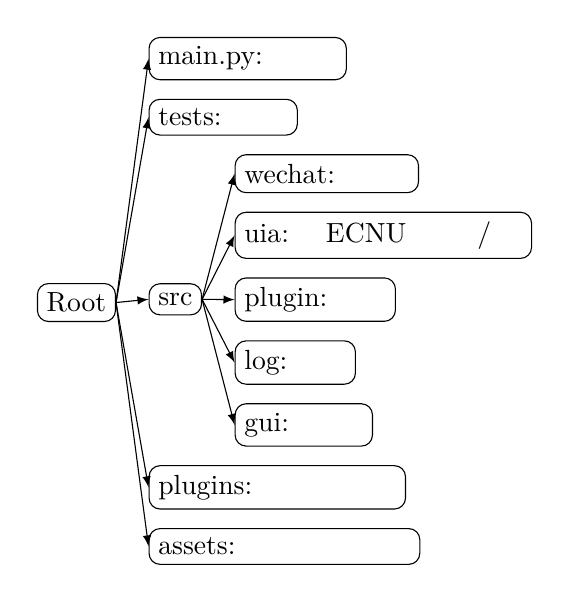
\begin{tikzpicture}
            % 绘制项目结构的树状图
            \node at (0, 0) {
                \begin{forest}
                    for tree={
                        grow=east,
                        draw,
                        edge={-latex},
                        rounded corners,
                        node options={align=center},
                        anchor=west,
                        parent anchor=east,
                        child anchor=west,
                        delay={where content={}{shape=coordinate}{}} % 避免错误节点
                    }
                    % @formatter:off
                    [Root
                        [assets: 静态资源目录,包含各开发参考文件及图标等。]
                        [plugins: 各个插件具体实现,可单独删除和添加
                            % todo 记得填写插件一句话简介
                        ]
                        [src
                            [gui: 实现图形用户界面]
                            [log: 实现日志输出]
                            [plugin: 实现插件架构]
                            [uia: 实现 ECNU 统一身份认证辅助/自动登录]
                            [wechat: 实现微信自动控制]
                        ]
                        [tests: 项目早期测试集]
                        [main.py: 软件启动入口文件]
                    ]
                    % @formatter:on
                \end{forest}
            };
        \end{tikzpicture}
    \end{center}

    \newpage{}


    \section{项目详述}\label{sec:project-desc}
    插件许多功能需要调用 ECNU 提供的各种接口。
接口的调用依赖于 ECNU 各个系统的登录缓存(在项目内部保存为 \verb`LoginCache`)。
为了获取有效的登录缓存简化登录操作,
插件登录使用了 WebDriver 控制浏览器实现自动化或半自动化的辅助登录流程。

在插件登录时,会出现浏览器 ECNU 统一身份认证的界面,登录有两种方式。
\begin{itemize}
    \item 方法一:填写图\ref{fig:uia-login-form} 中的表单实现登录。
    \item 方法二:扫描图\ref{fig:uia-login-qrcode} 中的二维码实现登录。
\end{itemize}

\begin{table}[H]
    \centering
    \begin{tabular}{cc}
        \begin{minipage}[H]{0.5\textwidth}
            \centering
            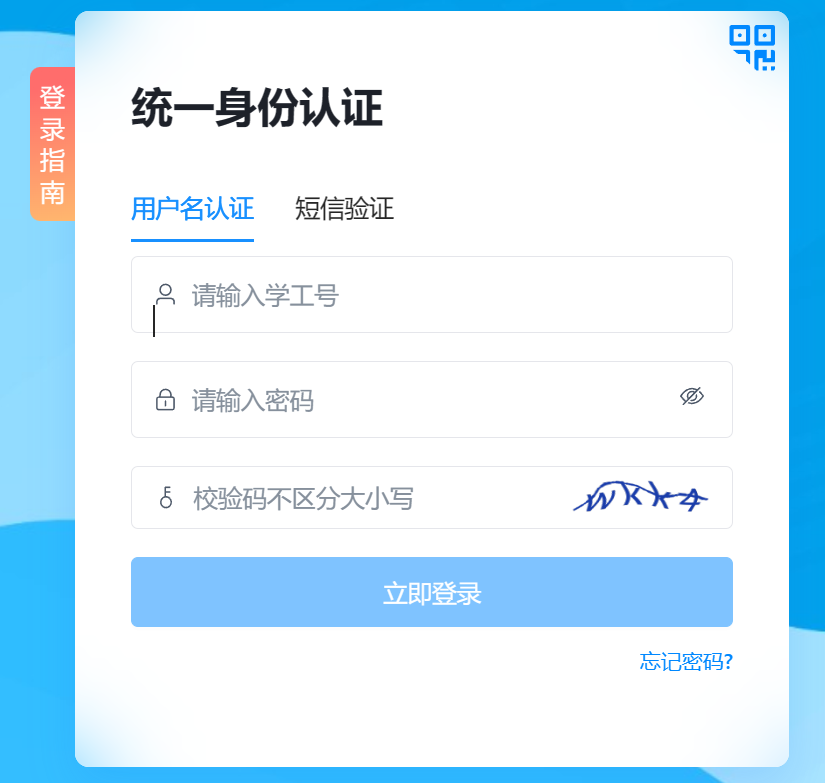
\includegraphics[width=0.8\textwidth]{img/uia_login_form}
            \captionof{figure}{ECNU UIA 登录界面(表单)}
            \label{fig:uia-login-form}
        \end{minipage} &
        \begin{minipage}[H]{0.5\textwidth}
            \centering
            
\includegraphics[width=0.8\textwidth]{img/uia_login_qrcode}
            \captionof{figure}{ECNU UIA 登录界面(二维码)}
            \label{fig:uia-login-qrcode}
        \end{minipage}
    \end{tabular}
\end{table}

\begin{rmr}[切换表单登录和二维码登录]
    \quad 表单登录:
    可以在项目根目录创建文件 \verb`login_info.toml`
    然后填写如下内容(替换尖括号以内的部分)。
    插件登录时会读取此文件中的学号密码,自动填写图\ref{fig:uia-login-form} 中的表单,实现全自动辅助登录。
    % @formatter:off
    \begin{verbatim}
stu_number = "<填写学号>"
password = "<填写数据库密码>" \end{verbatim}
    % @formatter:on

    \quad 二维码登录:
    删除 \verb`login_info.toml` 文件,
    此时插件辅助登录时会截取二维码图片并发送至邮箱提醒(如果已配置 \verb`email_notifier` 插件,见\ref{plugin-email-notifier})。 % todo 完成这个插件的介绍
    可以使用微信扫描二维码或用微信打开邮件中的连接实现半自动登录。
\end{rmr}

\subsubsection{辅助登录大致实现}

当此软件执行辅助登录的时候:

\begin{description}
    \item[二维码登录]
    进入 ECNU 统一身份认证(下面简称 UIA)界面之后,辅助登录默认使用二维码登录而不是表单登录。
    二维码登录时,脚本截取 UIA 二维码登录图片然后发送到目标邮箱,通过用户微信扫描二维码或者微信打开邮箱中的连接来实现登录。
    \item[表单登录]
    如果创建了 \verb`login_info.toml` 文件(步骤见上述提示),那么脚本会读取其中的学号和密码并自动填写到 UIA 表单中。
    表单中的验证码通过开源库 \hyperref{https://github.com/sml2h3/ddddocr}{DDDDocr} 来识别,成功识别四位验证码之后模拟点击登录按钮来登录。
    如果验证码识别失败则刷新重试。
\end{description}

成功登录 UIA 之后,各个插件通过自己实现的缓存抓取函数(\textit{Cache Grabber})在各个 ECNU 系统中获得所需要的登录缓存。

最终,登录缓存通过插件加载器(\textit{Plugin Loader})分发给各个插件。
    \newpage{}

    \subsection{研修间预约模块}

    \subsubsection{代码框架及分析}

    此部分代码位于 \texttt{src/studyroom/} 中。

    \begin{figure}[H]
        \centering
        \resizebox{\textwidth}{!}{
            \begin{minipage}[H]{0.5\textwidth}
                \centering
                \begin{forest}
                    for tree={
                        grow=east,
                        draw,
                        edge={-latex},
                        rounded corners,
                        node options={align=center},
                        anchor=west,
                        parent anchor=east,
                        child anchor=west,
                        delay={where content={}{shape=coordinate}{}} % 避免错误节点
                    }
                    [root
                    [src
                    [studyroom
                    [\_\_init\_\_.py]
                    [available.py]
                    [query.py]
                    [reserve.py]
                    ]
                    ]
                    [tests
                    [test\_studyroom
                    [available.py]
                    [query.py]
                    [reserve.py]
                    ]
                    ]
                    ]
                \end{forest}
            \end{minipage}

            \hspace{0.8cm}

            \begin{minipage}[H]{0.45\textwidth}
                \raggedright
                \textbf{模块说明:}\\
                \vspace{0.2cm}
                \textbf{Query (\texttt{query.py})}\\
                该模块仅实现对 \texttt{url} 的简单请求,不作任何数据处理。它通过相应的 API 获取研修室的可用性和详细信息。\\
                \vspace{0.4cm}

                \textbf{Available (\texttt{available.py})}\\
                \texttt{available.py} 模块负责处理房间可用性数据。它分析当前和已预订的时间段,确定研修室可预约的时间段。\\
                \vspace{0.4cm}

                \textbf{Reserve (\texttt{reserve.py})}\\
                \texttt{reserve.py} 模块管理预约流程。它包括进行预约、检查预约状态以及在特定条件下自动取消预约的功能。
            \end{minipage}
        }
        \caption{研修间的目录结构及模块说明}
        \label{fig:directory_structure}
    \end{figure}

    \subsubsection{研修间预约实现原理}

    华东师范大学研修间预约最少预约时长在 60 分钟以上,采用贪心思想,我们尽量预约更长的时间段以供使用,即使不能使用还可以及时离开。

    查看研修间的预约情况,我们首先需要计算出可用时间都有哪些:

    \begin{figure}[H]
        \centering
        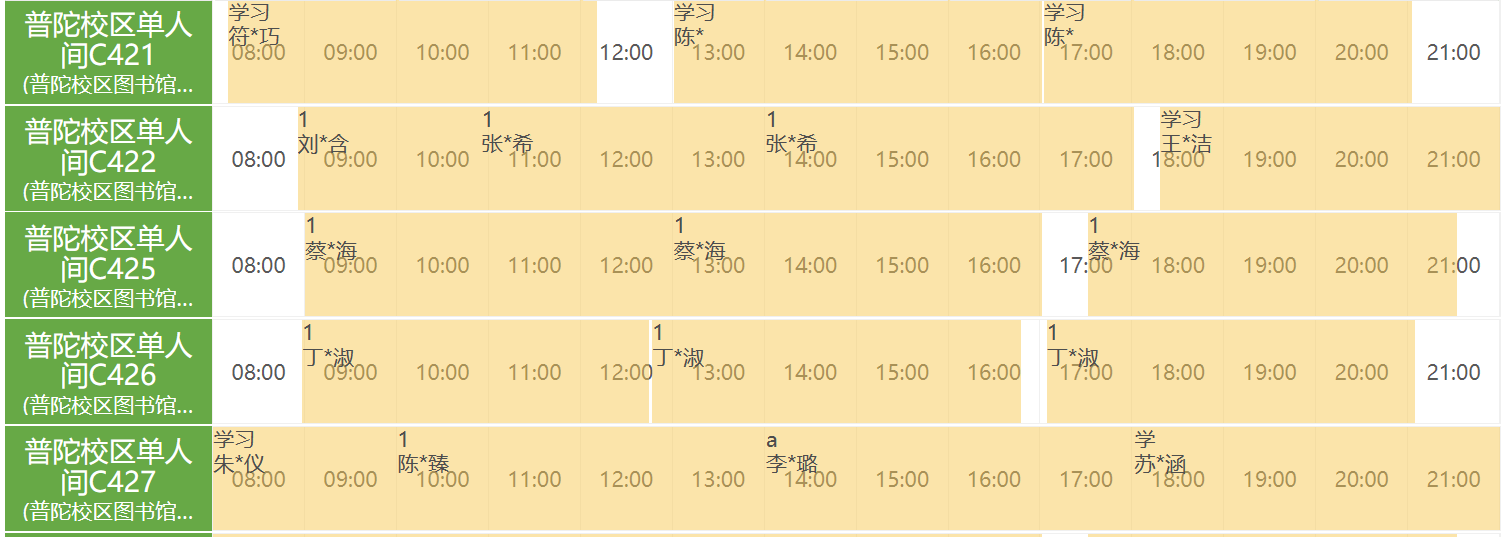
\includegraphics[width=0.62\textwidth]{img/studyroom_state.png}
        \caption{研修间状态示例}
        \label{fig:studyroom_available}
    \end{figure}

    研修间预约时,需要提交的表单样式如下,我们不采用浏览器自动操作的形式,而是截取提交时发送的 url 请求:

    \begin{figure}[H]
        \centering
        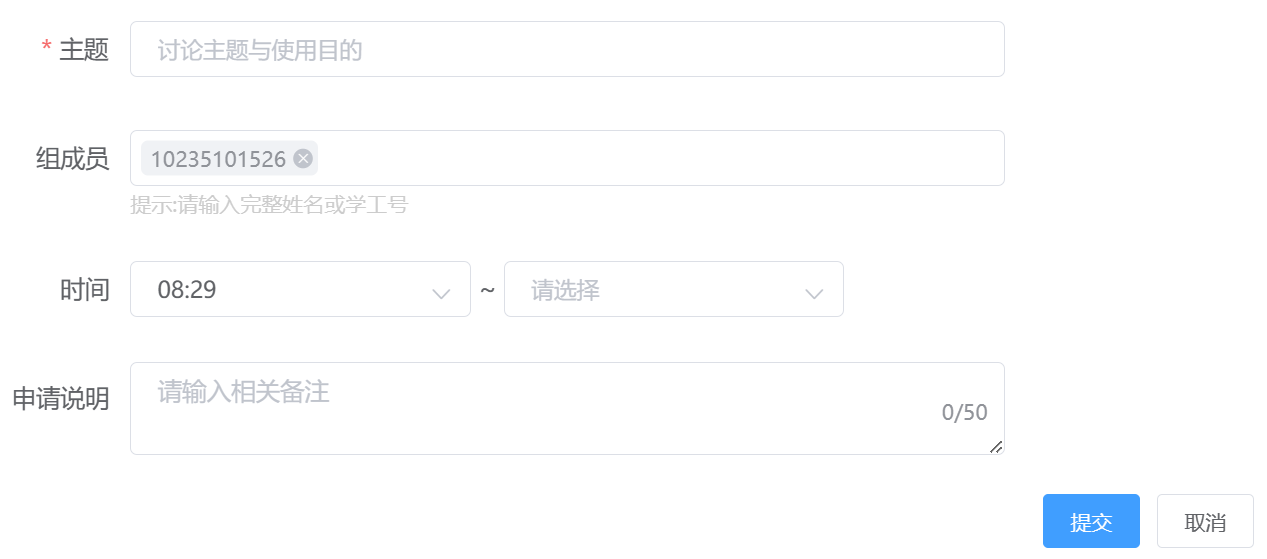
\includegraphics[width=0.5\textwidth]{img/studyroom_submit.png}
        \caption{研修间预约表单}
        \label{fig:studyroom_reserve}
    \end{figure}

    抓包得到 POST 请求的 Url 如下:\href{https://studyroom.ecnu.edu.cn/ic-web/reserve}{\underline{https://studyroom.ecnu.edu.cn/ic-web/reserve}}

    只需传入相关的字段即可:

    \begin{figure}[H]
        \centering
        \begin{minipage}[H]{0.45\textwidth} % 左侧放图片
            \centering
            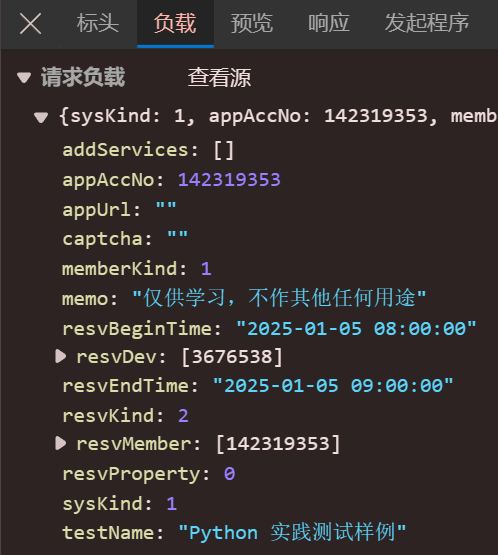
\includegraphics[width=0.6\textwidth]{img/studyroom_request.png}
            \caption{研修间预约请求}
            \label{fig:studyroom_request}
        \end{minipage}
        \hspace{0.05\textwidth} % 图片和代码之间的间距
        \begin{minipage}[H]{0.4\textwidth} % 右侧放代码
            \centering
            \begin{lstlisting}[language=python, caption={预约请求需要传入的字段}, label={lst:studyroom_request}]
headers = {
    "Cookie": f"ic-cookie={ic_cookie}", 
} # 从 StudyroomCache 中获取 ic-cookie

# 从 _fetch_userInfo 获取用户 ID
appAccNo = self._fetch_userInfo().get("accNo")

payload = {
    "sysKind": 1,  # 系统类型,默认为 1
    "appAccNo": appAccNo,
    "memberKind": 1,  # 成员类型,默认为 1
    "resvBeginTime": resvBeginTime,
    "resvEndTime": resvEndTime,
    "testName": testName,
    "resvMember": [appAccNo],
    # 默认预约人员列表只有当前用户
    "resvDev": resvDev,
    "memo": memo,
}
            \end{lstlisting}
        \end{minipage}
    \end{figure}

    加载入网页时,我们抓包发现,URL:\href{https://studyroom.ecnu.edu.cn/ic-web/roomDevice/roomAvailable}{\underline{URL: https://studyroom.ecnu.edu.cn/ic-web/roomDevice/roomAvailable}}
    拥有查询当前类别的研修间的功能,其返回的字段如下:

    \begin{lstlisting}[language=python]
    {'devId': 3676503,                             # 设备 ID
    'devName': '普陀校区单人间C421',                # 设备名称
    'minResvTime': 60,                             # 最小预约时间
    'openTimes': [{'openEndTime': '22:00',         # 开放结束时间
                   'openLimit': 1,                 # 最少预约人数
                   'openStartTime': '08:00'}],     # 开放开始时间
    'resvInfos': [{'resvBeginTime': '2024-12-26 '  # (People No.1) 的预约信息
                                    '17:01:00',
                   'resvEndTime': '2024-12-26 '
                                  '21:01:00',
                   'resvStatus': 1093}]},
    \end{lstlisting}

    它只为我们提供了 \texttt{'resvInfos'} 字段,这应该是用于前端供渲染黄色已预定时间段的给用户的,
    所以我们需要将它与 \texttt{'openTimes'} 字段结合起来,得到研修室的可用时间段。

    \begin{note}
        \begin{itemize}
            \item 将 [openStartTime, currentTime] 区间视为不可用时间段。例如当天 18:55 P.M 前的时间段都无效。
            \item 仅 AvailableTime > minResvTime 时,才将这段区间设置为 AvailableTime, 如果不超过最小预约时间,则不予考虑。
        \end{itemize}
    \end{note}

    返回的信息字典中,我们通过程序包含了一个新字段 \texttt{availableInfos},这样就可以提供给用户可用的时间段了。

    之后,使用 \texttt{reserve.py} 中的函数 \texttt{\_fetch\_userInfo} 来获取 \texttt{appAccNo},这是识别用户身份的字段,
    在发送 \texttt{reserve} 请求时,需要传入该字段作为 Payload 的一部分。最后通过调用 \texttt{reserve\_room} 函数即可完成全自动预约。

    \begin{note}
        每一次预约都会形成一个唯一的预约编号,称为 \texttt{uuid},我们在进入个人中心时,网页会自动调用查询的接口:

        \href{https://studyroom.ecnu.edu.cn/#/ic/userinfo}{\underline{https://studyroom.ecnu.edu.cn/\#/ic/userinfo}}
        ,所以,我们也可以通过抓包获取 uuid,便可以知道用户当前是否有预约了,这为后续的自动取消预约提供了保障。
    \end{note}

    \subsection{图书馆预约模块}

    \subsubsection{代码框架及分析}

    \begin{figure}[H]
        \centering
        \resizebox{\textwidth}{!}{
            \begin{minipage}[H]{0.5\textwidth}
                \centering
                \begin{forest}
                    for tree={
                        grow=east,
                        draw,
                        edge={-latex},
                        rounded corners,
                        node options={align=center},
                        anchor=west,
                        parent anchor=east,
                        child anchor=west,
                        delay={where content={}{shape=coordinate}{}} % Avoid empty nodes
                    }
                    [root
                    [plugins
                    [library
                    [\_\_init\_\_.py]
                    [date.py]
                    [encrypt.py]
                    [library\_plugin.py]
                    [query.py]
                    [req.py]
                    [seat.py]
                    [subscribe.py]
                    [tests.py]
                    ]
                    ]
                    ]
                \end{forest}
            \end{minipage}

            \hspace{0.8cm}

            \begin{minipage}[H]{0.45\textwidth}
                \raggedright
                \textbf{模块说明:}\\

                \textbf{Date (\texttt{date.py})}\\
                负责处理日期相关功能,例如格式化和时间操作。\\
                \vspace{0.4cm}

                \textbf{Encrypt (\texttt{encrypt.py})}\\
                提供加密和解密功能,用于数据传输安全。\\
                \vspace{0.4cm}

            \end{minipage}
        }
        \caption{ECNU 图书馆预约模块说明}
        \label{fig:directory_structure}
    \end{figure}

    \subsubsection{图书馆预约实现原理}

    \subsection{课前提醒模块}

    \subsubsection{代码框架及分析}

    \subsubsection{课表获取及数据处理原理}

    \begin{table}[H]
        \centering
        \begin{tabular}{cc}
            \begin{minipage}[H]{0.4\textwidth}
                \centering
                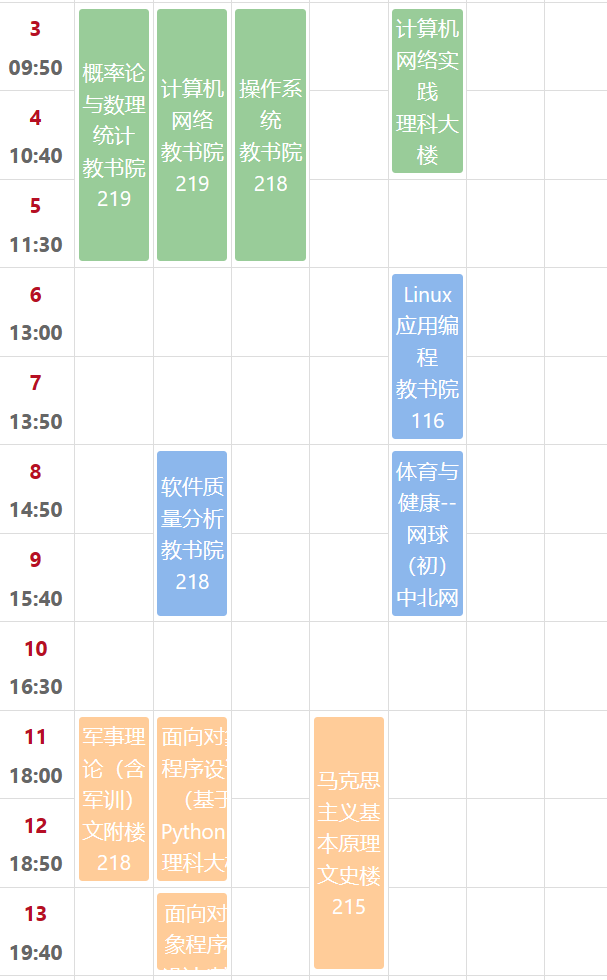
\includegraphics[width=0.5\textwidth]{img/calendar.png}
                \captionof{figure}{ECNU Portal 课表页面}
                \label{fig:login}
            \end{minipage} &
            \begin{minipage}[H]{0.5\textwidth}
                \raggedright
                \begin{rmr}
                    进入电脑端 Portal 主页面右侧,我们可以看到自己的课表,使用抓包工具得知,实际上,本课表是存在一个请求 url 的。

                    \vspace{0.5cm}

                    那么我们通过上述获得的 \texttt{login\_cache},通过 requests 库发起请求,即可实时获取课表。
                \end{rmr}
            \end{minipage}
        \end{tabular}
    \end{table}

    \begin{figure}[H]
        \centering
        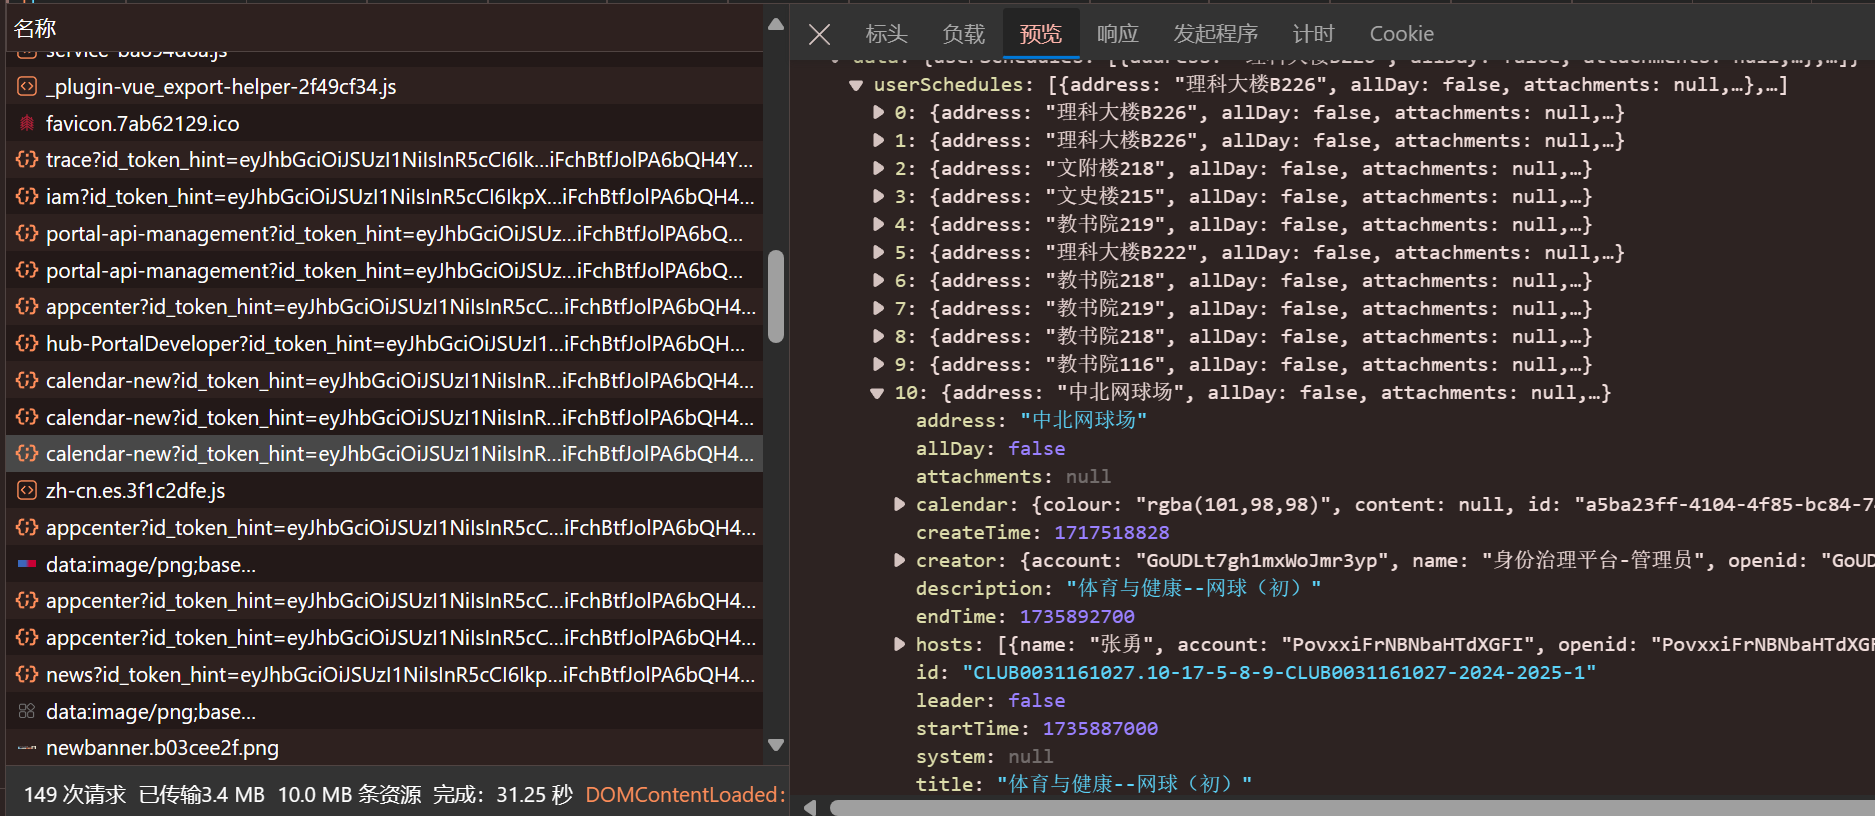
\includegraphics[width=0.8\textwidth]{img/calendar-new-url.png}
        \caption{Portal 课表请求}
        \label{fig:portal_course_table}
    \end{figure}

    这个 POST 请求采用的是 GraphQL 的查询格式,我们只需要使用 filter 过滤器查询自己所需要的字段即可。

    \begin{lstlisting}[language=python]
    USER_SCHEDULES = """
    query ($filter: ScheduleFilter, $userId: String) {
      userSchedules(filter: $filter, userId: $userId) {
        address # 上课地点
        hosts {
          name # 教师名字
        }
        description # 课程信息和描述
        endTime # 结束时间
        startTime # 开始时间
      }
    }
    """
    \end{lstlisting}

    我们原定的设计是查询当前时刻至次日该时刻,用户的课程安排,如果有课程,上课前的一定时段发送邮件提醒用户去上课。
    可以通过插件配置来配置上课前多久提醒用户,相关内容在后面进行详述。

    \begin{rmr}
        该功能配置一次后,便可以在后台轮询调用,
        后续我们考虑加入手机端的定位功能,查询用户是否已经到达指定的上课地点,便不发送邮件。
    \end{rmr}

    \newpage{}

    \subsection{插件装载(PluginLoader)模块}

    \subsubsection{Cache 分发}


    \begin{figure}[H]
        \centering
        \begin{minipage}[H]{0.45\textwidth}
            \centering
            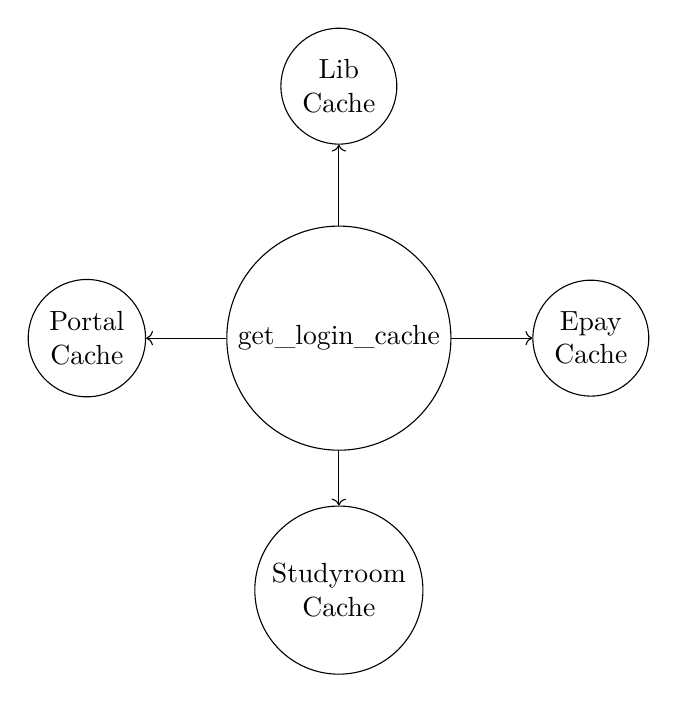
\begin{tikzpicture}[
                node distance=3.2cm,
                every node/.style={draw, circle, minimum size=1.2cm, align=center},
                every edge/.style={draw, thick, -{Latex[length=2mm, width=1mm]}}
            ]

                \node[draw] (center) {get\_login\_cache};

                \node[above of=center] (top) {Lib \\ Cache};
                \node[below of=center] (bottom) {Studyroom \\ Cache};
                \node[left of=center] (left) {Portal \\ Cache};
                \node[right of=center] (right) {Epay \\ Cache};

                \draw[->] (center) -- (top);
                \draw[->] (center) -- (bottom);
                \draw[->] (center) -- (left);
                \draw[->] (center) -- (right);

            \end{tikzpicture}
        \end{minipage}
        \hfill
        \begin{minipage}[H]{0.5\textwidth}
            \textbf{PluginLoader 缓存分发功能}:
            \begin{itemize}
                \item \textbf{Lib Cache}:用于图书馆管理系统。
                \item \textbf{Studyroom Cache}:用于研修间自动预约系统。
                \item \textbf{Portal Cache}:用于公共数据库页面的缓存,目前仅用于课表的获取。
                \item \textbf{Epay Cache}:用于华东师范大学校园卡管理页面的自动查询电费功能。
                \item \textbf{More Cache...}:适配的框架可以获取其余 ECNU 页面的 Cache 以供开发者使用。
            \end{itemize}
            \textbf{功能说明}:
            PluginLoader 是一个插件管理器,它可以加载、卸载和管理插件。
            通过调用 \texttt{get\_login\_cache()} 函数,PluginLoader 实现各缓存的分发,
            各缓存分发后供相应的插件调用。

            \vspace{0.2cm}

        \end{minipage}
    \end{figure}

    \begin{rmr}
        \textbf{更多适配}:
        我们已经实现了基本的 Cache 抓取框架,以供后续的开发者调用,调用示例如下:

        \texttt{get\_login\_cache(cache\_grabbers=[\{MoreCache\}.grab\_from\_driver])}
    \end{rmr}

    除此之外,每一个插件都拥有自己的 Routine 事件周期,Plugin 在注册时需要附带该属性,
    以保证 PluginLoader 能够轮询执行插件的例行任务(通过 PluginLoader 中定义的 \texttt{poll()} 函数来执行)。

    \subsubsection{基于 Routine 的事件调度逻辑}

    \begin{note}
        \noindent \textbf{PluginLoader} 根据预定义的频率(Secondly、Minutely、Hourly、Daily、Weekly),调用每个插件的 \texttt{on\_routine} 方法。插件会根据任务频率接收并处理任务,完成对应的功能逻辑。

        \vspace{0.3cm}

        \noindent 箭头上的 "Routine" 统一表示调度逻辑,具体任务频率的细节由配置文件决定。例如:
        \begin{itemize}
            \item \texttt{Routine: Secondly} → 调用 插件 A 的 \texttt{on\_routine}。
            \item \texttt{Routine: Daily} → 调用 插件 D 的 \texttt{on\_routine}。
        \end{itemize}
    \end{note}

    \vspace{0.27cm}

    \begin{center}
        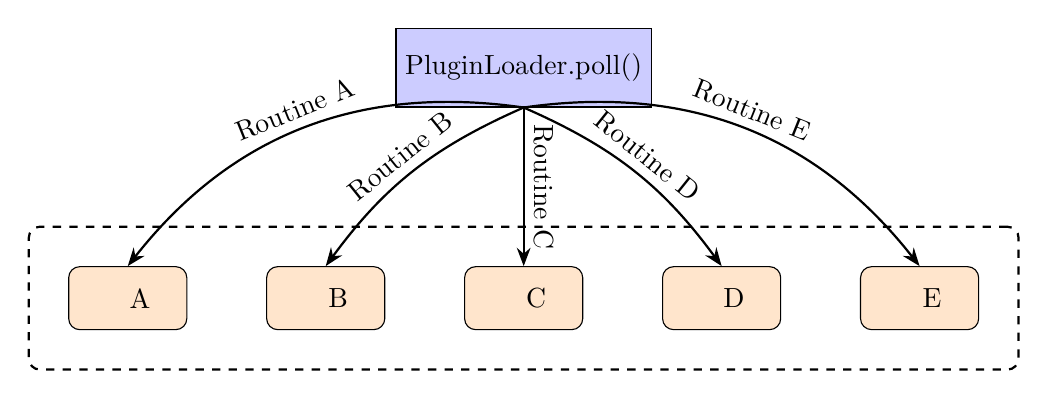
\begin{tikzpicture}
            [
            plugin/.style={
                rectangle,
                draw,
                rounded corners,
                fill=orange!20,
                minimum width=1.5cm,
                minimum height=0.8cm,
                align=center
            },
            loader/.style={
                rectangle,
                draw,
                fill=blue!20,
                minimum width=3cm,
                minimum height=1cm,
                align=center
            },
            dashedbox/.style={
                draw,
                dashed,
                thick,
                rounded corners,
                inner sep=0.5cm
            },
            arrow/.style={
                ->,
                thick,
                >=Stealth
            }
            ]
            % 定义插件节点,水平排列
            \node (A) [plugin] {插件 A};
            \node (B) [plugin, right=of A] {插件 B};
            \node (C) [plugin, right=of B] {插件 C};
            \node (D) [plugin, right=of C] {插件 D};
            \node (E) [plugin, right=of D] {插件 E};

            % 使用 fit 库创建包裹插件的虚线框
            \node [dashedbox, fit=(A) (E)] (dashedbox) {};

            % 将 PluginLoader 放置在虚线框正上方并居中
            \node (loader) [loader, above=1.5cm of dashedbox] {PluginLoader.poll()};

            % Draw curved arrows from PluginLoader to each plugin
            \draw[arrow, bend right=30] (loader.south) to node[midway, sloped, above] {Routine A} (A.north);
            \draw[arrow, bend right=15] (loader.south) to node[midway, sloped, above] {Routine B} (B.north);
            \draw[arrow] (loader.south) to node [midway, sloped, above] {Routine C} (C.north); % Straight arrow for the middle plugin
            \draw[arrow, bend left=15] (loader.south) to node [midway, sloped, above] {Routine D} (D.north);
            \draw[arrow, bend left=30] (loader.south) to node [midway, sloped, above] {Routine E} (E.north);

        \end{tikzpicture}
    \end{center}

    \subsubsection{插件配置管理}

    \begin{note}
        此部分代码如 \texttt{root/src/plugin/config.py} 所示。

        我们使用装饰器来实现插件的注册,注册信息存储于 \texttt{Registry} 类的字典中,每个插件对应着一个 \texttt{Record} 对象。
    \end{note}

    示例性的插件注册代码如 \texttt{root/plugins/calendar\_notice.py} 中所示:

    \begin{lstlisting}[language=python]
    @register_plugin(
        name="calendar_notice",
        configuration=PluginConfig().add(
            TimeItem(
                name="notice_before_class_start", default_value=datetime.time(0, 10),
                description="上课提前提醒时间 (提前h小时m分钟)"
            )
        ),
        routine=Routine.MINUTELY,
        ecnu_cache_grabber=PortalCache.grab_from_driver
    )
    \end{lstlisting}

    文件中有 \texttt{PluginConfig} 和 \texttt{PluginContext} 类,它们的功能如下:

    \begin{itemize}
        \item \textbf{PluginConfig}:插件的配置项集合。插件可继承 \texttt{PluginConfig} 类并添加多个 \texttt{ConfigItem} 子类来描述其配置需求。
        \item \textbf{ConfigItem}:每个配置项通过继承 \texttt{ConfigItem} 类及其子类(如 \texttt{TextItem}、\texttt{NumberItem} 等)来定义。
    \end{itemize}

    \textbf{功能说明}:PluginConfig 提供了一种结构化的方式来定义插件的配置项,支持配置项的序列化和反序列化,方便配置的保存和加载。
    插件在注册时通过 \texttt{PluginConfig} 指定其需要的配置项,框架会自动处理配置的管理。

    \begin{figure}[H]
        \centering
        \resizebox{0.4\textwidth}{!}{
            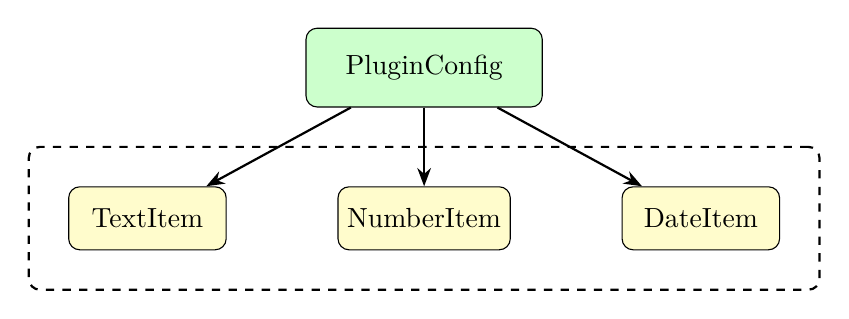
\begin{tikzpicture}
                [
                pluginconfig/.style={ rectangle, draw, rounded corners, fill=green!20, minimum width=3cm, minimum height=1cm, align=center },
                configitem/.style={ rectangle, draw, rounded corners, fill=yellow!20, minimum width=2cm, minimum height=0.8cm, align=center },
                dashedbox/.style={ draw, dashed, thick, rounded corners, inner sep=0.5cm },
                arrow/.style={ ->, thick, >=Stealth }
                ]
                \node (pluginconfig) [pluginconfig] {PluginConfig};
                \node (textitem) [configitem, below left=of pluginconfig] {TextItem};
                \node (numberitem) [configitem, below=of pluginconfig] {NumberItem};
                \node (dateitem) [configitem, below right=of pluginconfig] {DateItem};

                \node [dashedbox, fit=(textitem) (numberitem) (dateitem)] (dashedbox) {};

                \draw[arrow] (pluginconfig) -- (textitem);
                \draw[arrow] (pluginconfig) -- (numberitem);
                \draw[arrow] (pluginconfig) -- (dateitem);

            \end{tikzpicture}
        }
        \caption{PluginConfig 和 ConfigItem 的关系示意图}
    \end{figure}

    \subsubsection{插件上下文管理}

    此部分代码见 \texttt{root/src/plugin/context.py} 所示。

    \begin{note}
        为了保证项目的整洁和规范性,插件创建文件和记录日志等操作请使用生命周期函数和事件函数中提供的 PluginContext 进行。
        它为每个插件提供了一个上下文环境,使插件能够与框架进行交互和访问必要的资源。
    \end{note}

    \begin{figure}[H]
        \centering
        \resizebox{0.95\textwidth}{!}{
            \begin{minipage}[H]{0.4\textwidth}
                \centering
                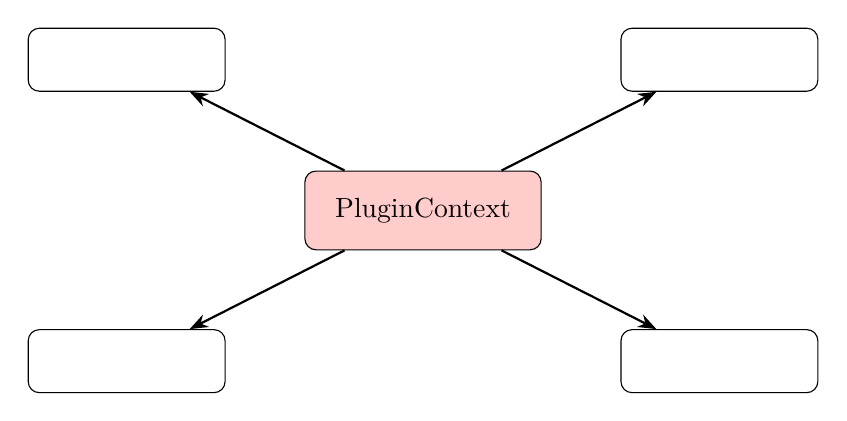
\begin{tikzpicture}
                    [
                    context/.style={
                        rectangle,
                        draw,
                        rounded corners,
                        fill=red!20,
                        minimum width=3cm,
                        minimum height=1cm,
                        align=center
                    },
                    feature/.style={
                        rectangle,
                        draw,
                        rounded corners,
                        fill=white!80,
                        minimum width=2.5cm,
                        minimum height=0.8cm,
                        align=center
                    },
                    arrow/.style={
                        ->,
                        thick,
                        >=Stealth
                    }
                    ]

                    % PluginContext Node
                    \node (context) [context] {PluginContext};

                    % Features of PluginContext
                    \node (logger) [feature, above left=of context] {日志记录器};
                    \node (cache) [feature, above right=of context] {插件缓存};
                    \node (message) [feature, below left=of context] {消息传递};
                    \node (actions) [feature, below right=of context] {用户操作绑定};

                    % Arrows from PluginContext to Features
                    \draw[arrow] (context) -- (logger);
                    \draw[arrow] (context) -- (cache);
                    \draw[arrow] (context) -- (message);
                    \draw[arrow] (context) -- (actions);

                \end{tikzpicture}
            \end{minipage}
            \hspace{2.5cm}
            \begin{minipage}[H]{0.6\textwidth}
                \textbf{PluginContext 的功能组成}:
                \begin{itemize}
                    \item \textbf{日志记录}:
                    插件专属的日志记录(信息、警告、错误等)。
                    \item \textbf{插件缓存}:
                    插件可以通过 \texttt{ctx.get\_cache()} 访问自己的持久化缓存,用于存储跨会话的数据。
                    缓存支持数据的读取和写入,确保插件状态的持久性。
                    \item \textbf{消息传递}:
                    允许插件间通信。
                    \item \textbf{用户操作绑定}:
                    插件可以绑定用户界面的操作(如按钮),相应的回调函数相应用户的操作。
                \end{itemize}
            \end{minipage}
        }
    \end{figure}

    \subsection{测试模块}

    在本项目中,我们采用了 Python 标准库中的 \texttt{unittest} 模块进行单元测试,以确保项目核心功能的稳定性和正确性。

    \begin{itemize}
        \item \textbf{测试环境的隔离}:通过 \texttt{setUp()} 和 \texttt{tearDown()} 方法,\texttt{unittest} 提供了对每个测试用例的独立初始化和资源回收,避免测试用例之间的相互干扰。
        \item \textbf{断言机制}:\texttt{unittest} 提供了多种断言方法(如 \texttt{assertEqual()}、\texttt{assertTrue()}),用以验证测试结果是否符合预期。
    \end{itemize}

    \textbf{测试用例的结构设计}:

    以下是测试模块的代码结构:
    \begin{lstlisting}[language=Python]
class TestCalendar(unittest.TestCase):
    def setUp(self):
        init()  # 初始化日志记录器
        self.cache = load_cache()  # 加载登录缓存
        self.calendar = CalendarQuery(self.cache.get_cache(PortalCache))

    def test_user_schedules(self):
        now = datetime.datetime.now()
        pprint(self.calendar.query_user_schedules(
            int(now.timestamp() * 1000),
            int((now + datetime.timedelta(days=1)).timestamp() * 1000),
        ))

    def test_school_calendar(self):
        school_calendar = self.calendar.query_school_calendar()
        pprint(school_calendar)
    \end{lstlisting}

    \textbf{测试框架的执行流程}:
    \begin{itemize}
        \item 在 \texttt{setUp()} 方法中完成初始化工作,包括日志系统的初始化和登录缓存的加载。
        \item 使用 \texttt{test\_user\_schedules()} 方法测试用户日程的获取功能,通过时间戳计算和校验确保数据范围的准确性。
        \item 使用 \texttt{test\_school\_calendar()} 方法验证校历的查询功能,确保校历数据的完整性和准确性。
    \end{itemize}

    \subsection{其他工具模块}

    \subsubsection{LateX 课表生成器}

    本模块位于 \texttt{root/tools/classtable} 之下。对应的测试文件为 \texttt{test/test\_latex}。

    在之前的课前提醒模块中,我们通过 GraphQL 的 filter 过滤器可以选中需要查询的时间戳,若要查询整个学期的课表,
    只需要将时间戳定于本周和下周即可,因为考虑到有一些课程是单周上的,这样能满足大部分人的需求。
    所以当我们获得了本周和下周的课表后,只需要做一次过滤,采用集合过滤法,指定一个字段作为 id,便能够实现两周课表的聚合。

    \begin{lstlisting}[language = python]
    seen = set()
    unique_classes = []
    for cls in double_week_class_table:
        # 创建唯一标识: (课程, 星期, 时间)
        identifier = (cls.title, weekday)
        if identifier not in seen:
            seen.add(identifier)
            unique_classes.append(cls)
        else:
            project_logger.info(f"去除重复课程: {cls.title} 在星期{weekday + 1} {class_time}")
    \end{lstlisting}

    然后按照 cls 给出的 \LaTeX 课表的格式,用 python 自动填充好,再使用 os 模块进行命令行编译即可。

    \begin{figure}[H]
        \centering
        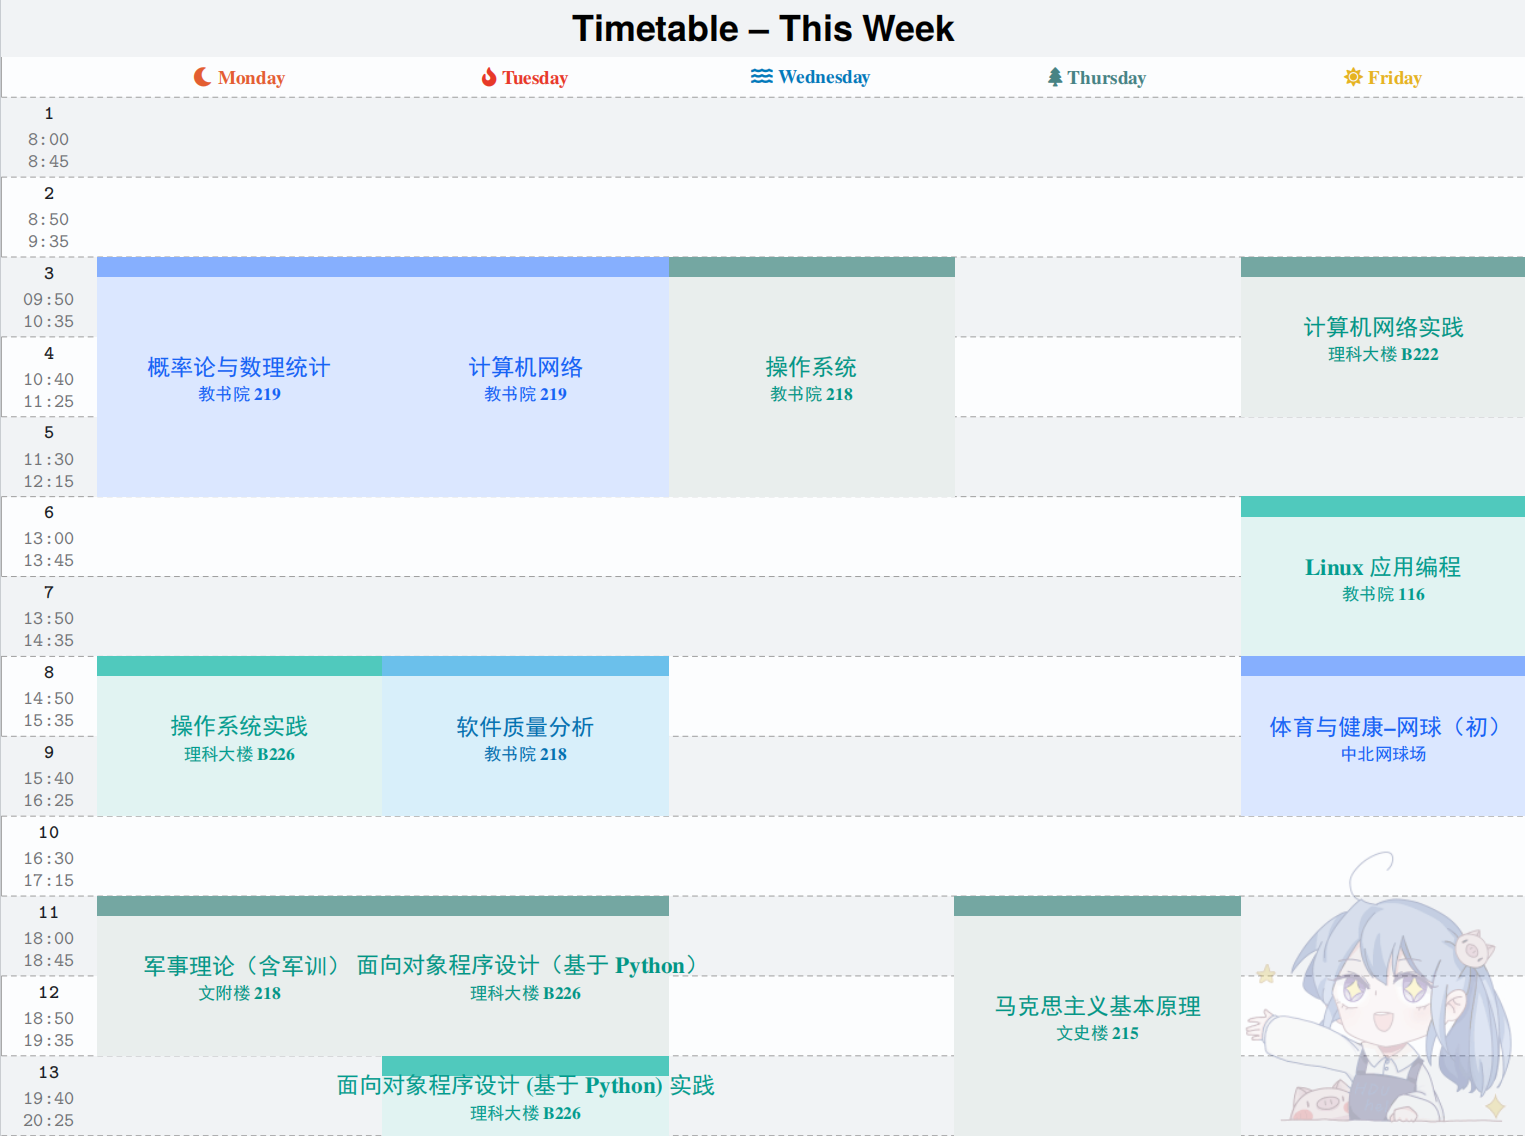
\includegraphics[width=0.6\textwidth]{img/classtable_example.png}
        \caption{LateX 课表生成示例}
        \label{fig:latex_table}
    \end{figure}

    \subsubsection{基于 CPP 实现文件复制到系统剪贴板}

    \begin{note}
        本模块位于 \texttt{src/cpp/copyfile\_build} 中。请查阅相关代码。

        我们使用 \texttt{CF\_HDROP} 数据格式进行 Windows 的文件复制入剪贴板,这一部分可参考 Microsort 写给开发者们的参考文档:
        \href{https://learn.microsoft.com/en-us/windows/win32/shell/clipboard#cf_hdrop}{\underline{https://learn.microsoft.com/en-us/windows/win32/shell/clipboard\#cf\_hdrop}}
    \end{note}

    \begin{figure}[H]
        \centering
        
\includegraphics[width=0.578\textwidth]{img/CF_HDROP.png}
        \caption{Microsoft Study Doc - CF\_HDROP}
        \label{fig:copyfile_to_clipboard}
    \end{figure}

    \textbf{CopyFileToClipboard} 函数是用来将一个文件路径复制到剪贴板的,基于 Windows API 实现。使用 \textbf{CF\_HDROP} 数据格式,它是 Windows 剪贴板的标准格式,用于表示文件路径。具体步骤:

    \begin{enumerate}
        \item 调用 \textbf{OpenClipboard} 打开剪贴板,清空剪贴板数据 (\textbf{EmptyClipboard})。
        \item 分配内存 (\textbf{GlobalAlloc}),创建一个 \textbf{DROPFILES} 结构体,其中存储文件路径。
        \item 使用 \textbf{GlobalLock} 锁定分配的内存并填充数据,调用 \textbf{SetClipboardData} 将文件路径放到剪贴板中。
        \item 最后释放内存并关闭剪贴板 (\textbf{CloseClipboard})。
    \end{enumerate}

    \subsubsection{微信交互接口}

    \begin{note}
        微信交互接口是我们最初的设计设想,Python 接管键鼠实现自动化办公,主要使用的是 uiautomation 库,
        它可以实现对 Windows 系统的 UI 自动化操作。

        \vspace{0.3cm}

        在项目中,我们实现了部分和微信有关的接口,能够为后续的开发者们提供逻辑参考。
        在此我们提供一个示例,将生成的 LaTeX 课表通过 CPP 文件复制到微信指定窗口并发送。
    \end{note}

    \vspace{0.2cm}

    \begin{forest}
        for tree={
            grow=east,
            draw,
            edge={-latex},
            rounded corners,
            node options={align=center},
            anchor=west,
            parent anchor=east,
            child anchor=west,
            delay={where content={}{shape=coordinate}{}} % 避免错误节点
        }
        [Root
        [src
        [wechat
        [\_\_init\_\_.py]
        [pc.py]
        [window.py]
        ]
        ]
        [tests
        [test\_wechat
        [test\_pc.py]
        [test\_window.py]
        ]
        ]
        ]
    \end{forest}

    \begin{itemize}
        \item \textbf{描述}: 封装微信的各种操作,如发送消息、图片、文件等。
        \item \textbf{方法}:
        \begin{enumerate}
            \item \texttt{open\_window()}: 唤起微信窗口并获取窗口控制对象。
            \item \texttt{close\_window()}: 关闭微信主窗口。
            \item \texttt{search(cls, pattern: str)}: 在微信搜索框中输入搜索内容并执行搜索。
            \item \texttt{locate\_chat(cls, name: str | None = None)}: 获取聊天窗口的输入框控件。
            \item \texttt{switch\_to(cls, name: str)}: 切换到指定名称的聊天窗口。
            \item \texttt{send\_message(cls, name: str, text: str)}: 向指定聊天对象发送文本消息。
            \item \texttt{send\_img(cls, name: str, img: str | typing.BinaryIO)}: 向指定聊天对象发送图片。
            \item \texttt{send\_file(cls, name: str, filepath: str)}: 向指定聊天对象发送文件。
        \end{enumerate}
    \end{itemize}


    \section{项目主要界面贴图}

    \subsection{基于 Pyside 6 的主界面}

    \subsection{插件配置页面}

    \subsection{托盘后台界面}

    通过运行 main.py 后,托盘中会出现一个图标,当鼠标悬停于其上时,可以查看当前的登录状态,使用鼠标右键退出该插件程序。

    \begin{figure}[H]
        \centering
        \begin{subfigure}[b]{0.35\textwidth}
            \centering
            
\includegraphics[width=0.8\textwidth]{img/tray_interface.png}
            \caption{处于任务栏的托盘}
            \label{fig:tray_interface}
        \end{subfigure}
        \hspace{0.06\textwidth}
        \begin{subfigure}[b]{0.3\textwidth}
            \centering
            
\includegraphics[width=\textwidth]{img/tray_exit.png}
            \caption{托盘退出按钮}
            \label{fig:tray_exit}
        \end{subfigure}
        \caption{托盘界面与退出按钮}
        \label{fig:tray_combined}
    \end{figure}


    \section{总结}

    \subsection{项目前景}

    本项目的开发过程是我们团队不断挑战自我、解决问题的过程。通过项目,我们不仅掌握了多个技术栈(如 Python 自动化、插件框架设计、C++ 系统调用等),还提高了团队的协作能力、代码规范性和需求分析能力。

    展望未来,本项目具备良好的扩展性,后续可以集成更多插件,覆盖更多校园生活场景。例如:
    \begin{itemize}
        \item 支持课表与日历软件(如 Google Calendar)的无缝同步。
        \item 集成更多校园生活服务,例如自动化导出成绩单、图书馆借阅管理、校园卡消费查询等。
    \end{itemize}

    通过持续迭代和优化,本项目有潜力为华东师范大学的师生带来更加便利的校园生活体验。

    \subsection{项目收获}

    \subsubsection*{关卓谦}

    \begin{Thought}
        在本项目中
    \end{Thought}

    \subsubsection*{张梓卫}

    \begin{Thought}
        我是本项目的组织者和相关 Idea 的提出者,也是该课程报告的主要撰写人,
        最初,我通过获取窗口 \texttt{PID} 实现了微信的简单接口,
        得益于良好的团队框架,后来使用团队中完善的 \texttt{Cache\_grabber} 框架,
        让我能够马上上手研修间预约模块的开发,熟悉了数据处理和 API 调用的结合应用,
        当然,LateX 课表生成器的开发让我对编译有了更深入的理解,

        \vspace{0.3cm}

        在不断翻看关卓谦的 \texttt{PluginLoader} 的代码到理解,最终写出一份详解的报告
        从提出到实现,从实现到推翻重来,一切都有迹可循。
        通过团队交流,我增强了自己的跨领域的开发编程能力,掌握了 Git 多种不同的使用方式,
        同时跟随团队的项目规范,掌握了如何通过良好的代码架构提高代码复用性和维护性。

        \vspace{0.3cm}

        同时,我还学到了如何利用 Python 的自动化工具(Selenium-Wire 和 requests)
        实现复杂的登录流程。翻看华东师范大学开发者文档时,涉及到鉴权,还了解到了 OAuth 2.0 和 JWT 等的认证机制。

        \vspace{0.3cm}

        是非常愉悦的一次项目经历!
    \end{Thought}

    \subsubsection*{王文锦}

    \begin{Thought}
        在本项目中
    \end{Thought}

    \subsection{注意事项}

    \begin{itemize}
        \item 本项目遵循 MIT 开源协议,\LaTeX 宏包部分使用 LPPL 授权。
        \item 华东师范大学校徽图案版权归华东师范大学所有。
        \item 项目使用 Pycharm 开发,课程报告使用 LaTeX 编写。
    \end{itemize}

    \subsection{参考资料}

    \begin{itemize}
        \item \href{https://learn.microsoft.com/en-us/windows/win32/shell/clipboard#cf_hdrop}{\underline{https://learn.microsoft.com/en-us/windows/win32/shell/clipboard\#cf\_hdrop}}
        \item \href{https://developer.ecnu.edu.cn/oauth2playground/}{\underline{https://developer.ecnu.edu.cn/oauth2playground/}}
        \item \href{https://github.com/sml2h3/ddddocr}{\underline{https://github.com/sml2h3/ddddocr}}。
        \item \href{https://developer.ecnu.edu.cn/vitepress/data/architecture/authorization.html}{\underline{https://developer.ecnu.edu.cn/vitepress/data/architecture/authorization.html}}
    \end{itemize}

\end{document}